\documentclass{article}

\usepackage[utf8]{inputenc}
\usepackage{graphicx}
\usepackage{float}

\usepackage{listings}
\lstset{
	basicstyle=\ttfamily,
	showstringspaces=false,
}
\setlength{\parindent}{0in} 

\title{App2 - Aufmass (Punkte und Geometrie)}
\date{\today}
\author{Matteo Togni, Florian Hausler}

\begin{document}
\clearpage\maketitle
\thispagestyle{empty}
\newpage

\subsection*{Ziel}
Das Ziel der App2 ist Administratoren Funktionalitäten für das Aufbauen der Geometrie (Points Of Interests und deren Verbindungen) anzubieten.


\subsection*{Stand der Entwicklung}
\label{subsubsec:stand}
Die Anwendung bietet an dem aktuellen Stand folgende Operationen an:
\begin{itemize}
  \item Anzeige der Liste der POIs
  \item Eintragen eines neues POI
  \item Aufnahme eines Bild fuer die einzelnen POIs
  \item Definieren direkter Verbindungen (ohne Umleitung) zwischen POIs (Checkbox "erreichbar"
\end{itemize}

\subsection*{Anwendungsfall: Definition einer neuen POI und deren Details}
\label{subsec:anwendungsfall_neuer_poi} 
Dem Benutzer wird die aktuelle Liste der POIs angezeigt (Bild 1).

\begin{figure}[H]
	\centering
	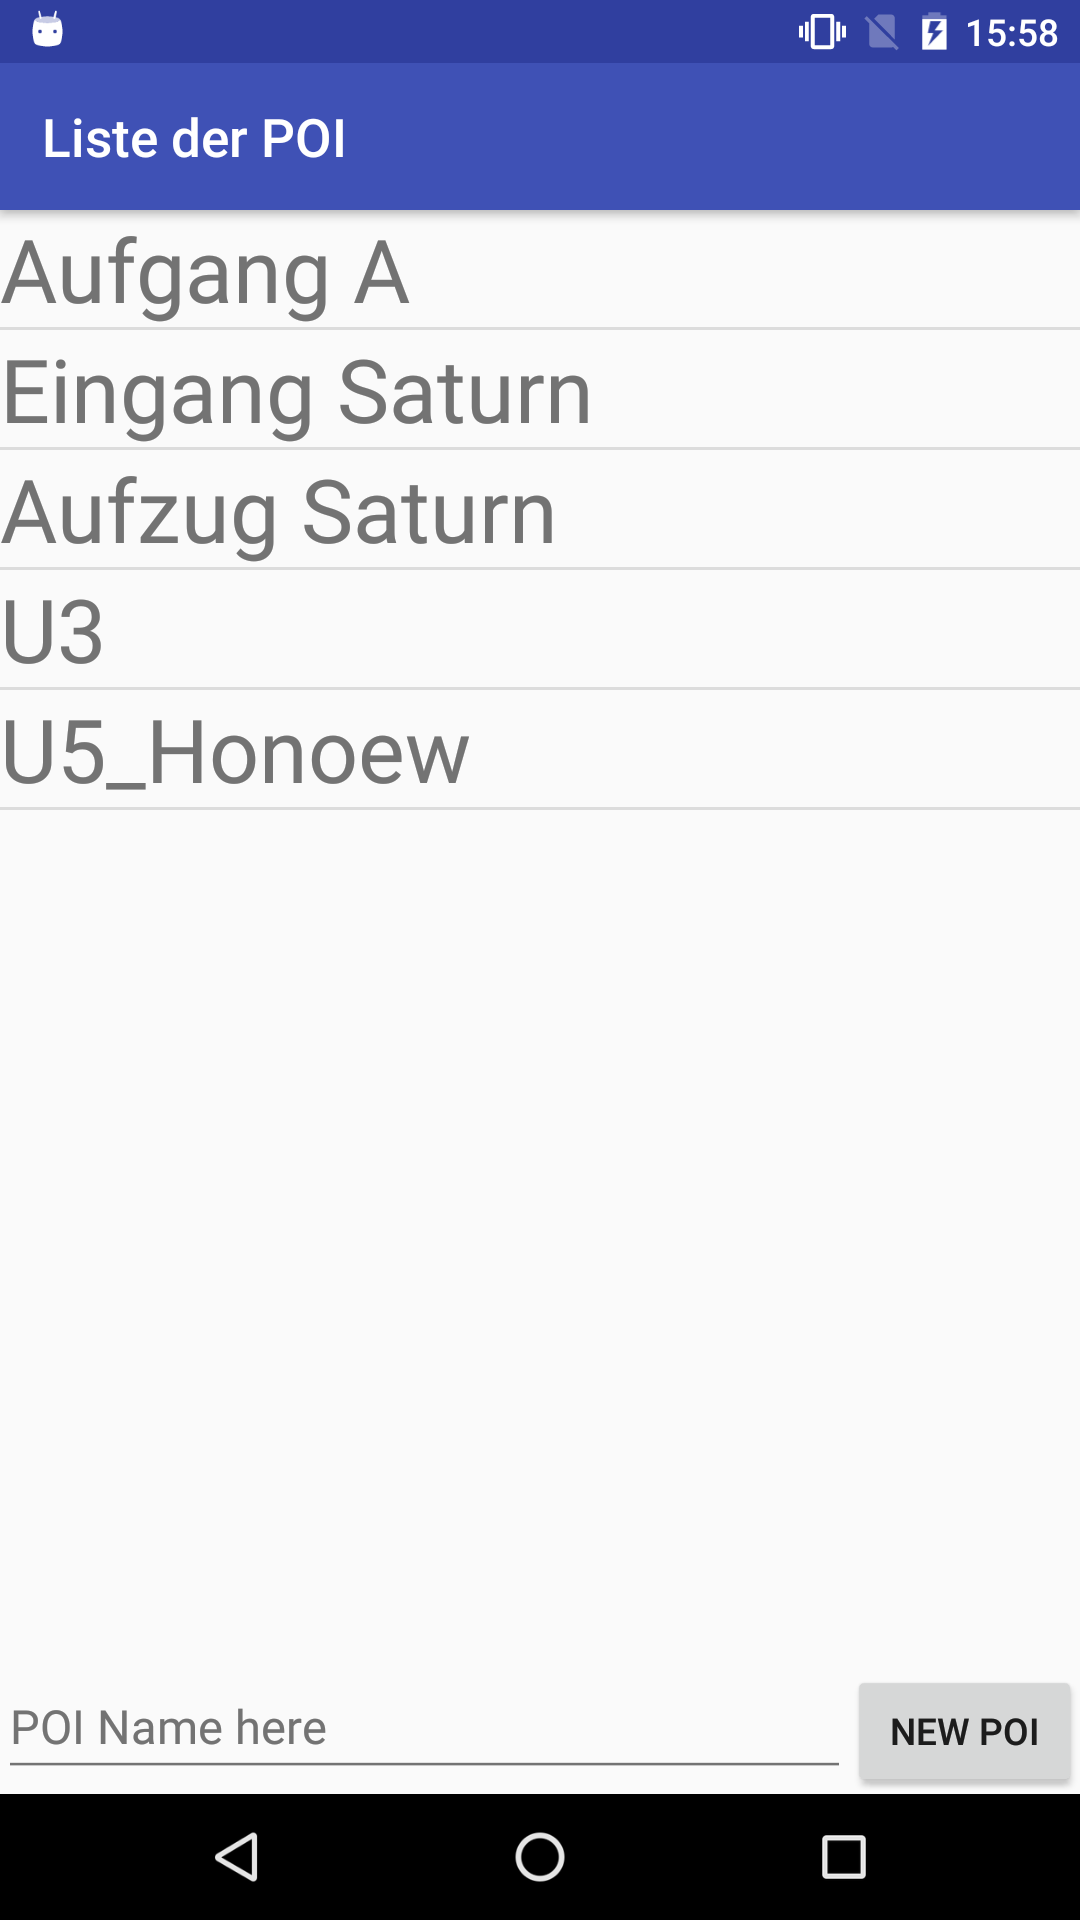
\includegraphics[scale=0.18]{images/poi_list_begin.png}
	\caption{Liste der POIs beim Ausführen der Anwendung}
	\label{fig:poi_list_begin}
\end{figure}

Der Benutzer ist in der Lage den Namen eines neuen POI mittels Tap auf der unterliegenden Eingabeschachtel zu definieren (Bild 2). 

\begin{figure}[H]
	\centering
	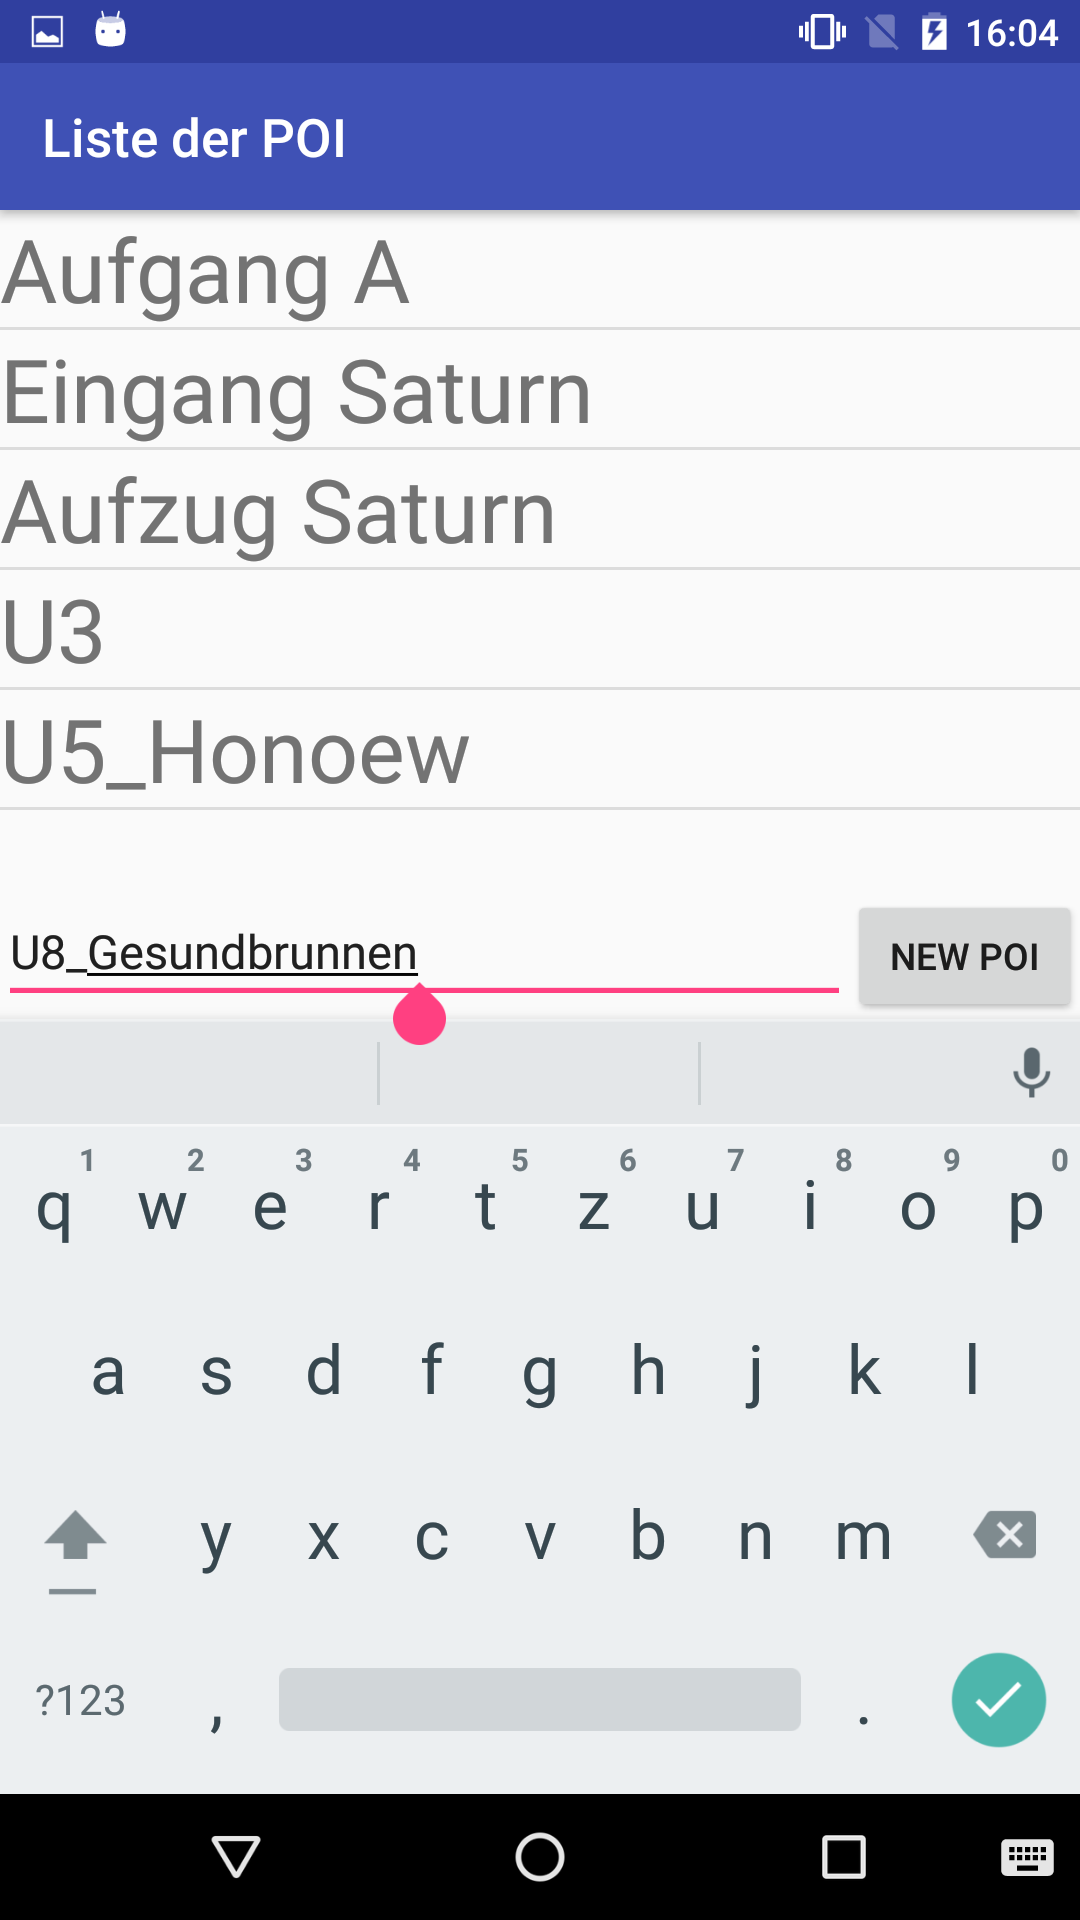
\includegraphics[scale=0.18]{images/poi_name_insert.png}
	\caption{Eingabe des neuen Namens}
	\label{fig:poi_name_insert}
\end{figure}

Durch Drucken auf dem "NEW POI" Knopf wird einen neuen POI erstellt und am Ende der obenen Liste angezeigt (Bild 3).

\begin{figure}[H]
	\centering
	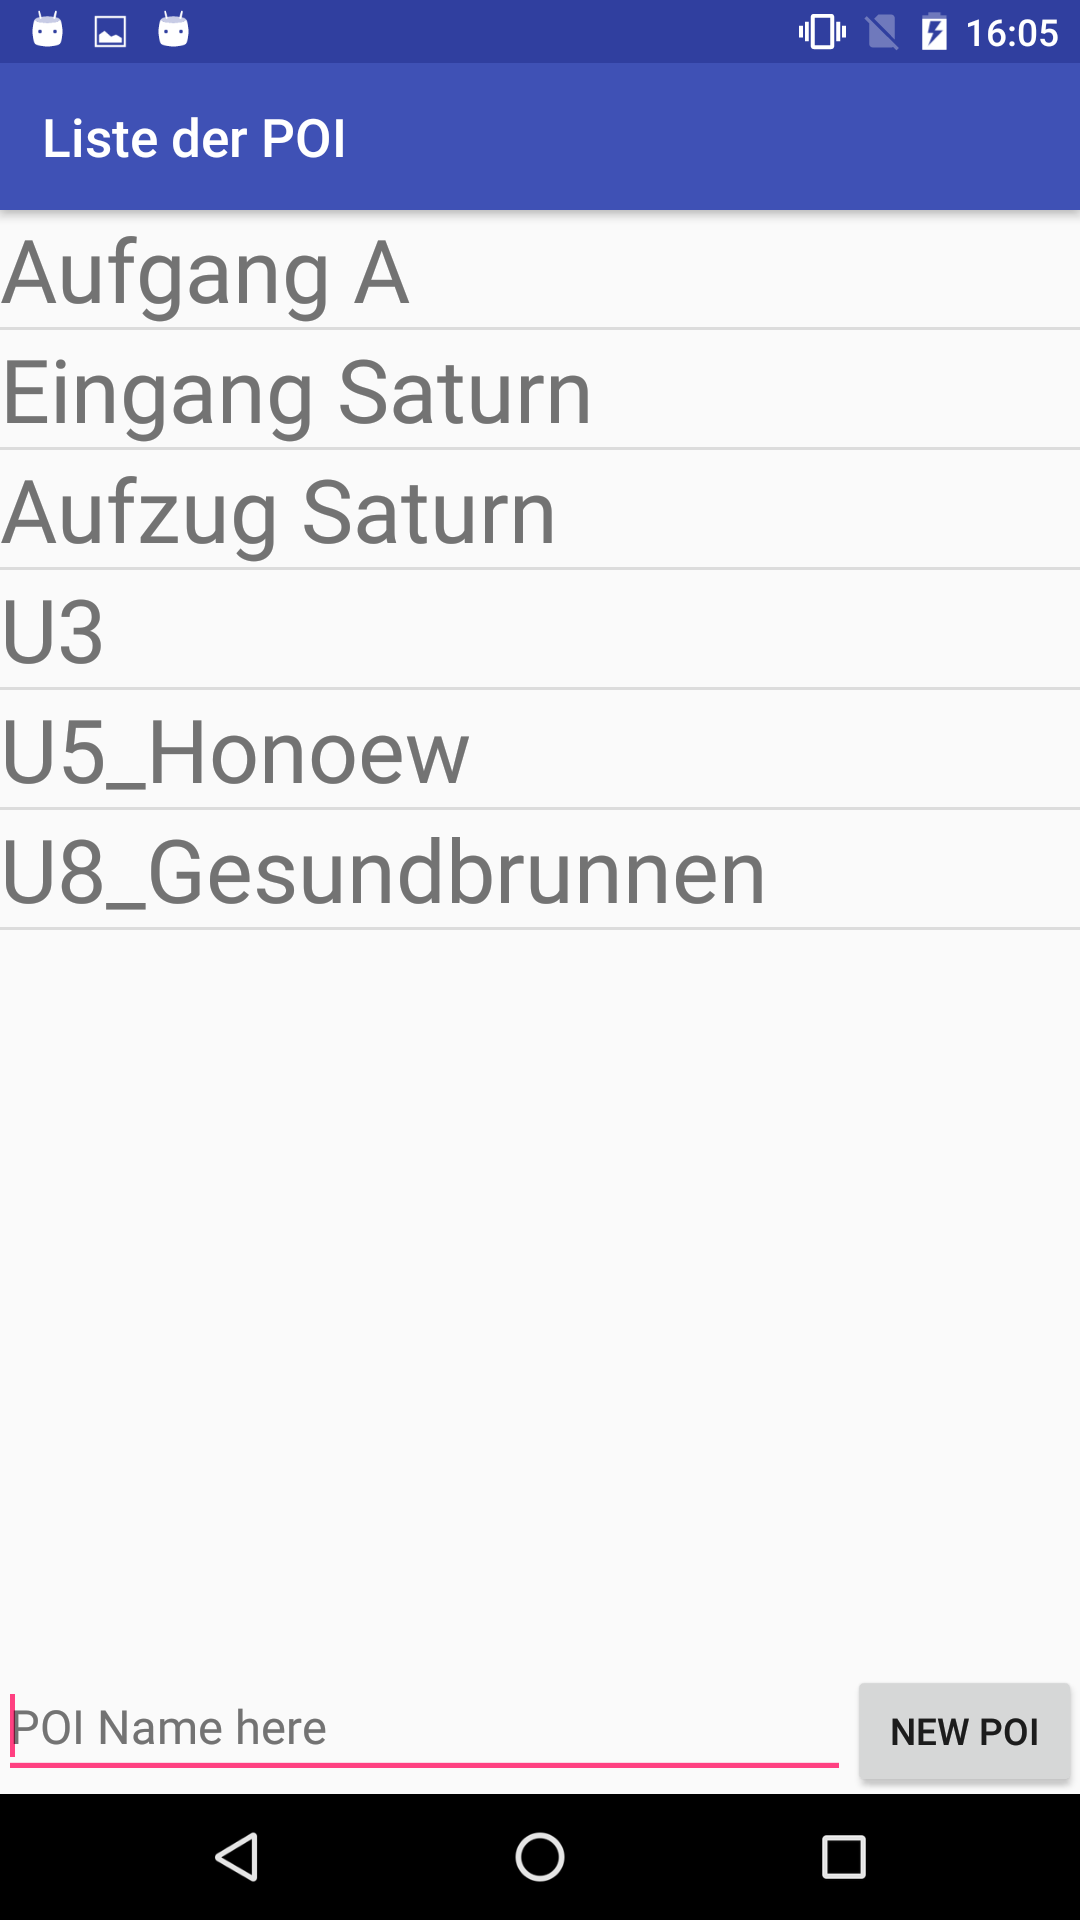
\includegraphics[scale=0.18]{images/poi_after_insertion.png}
	\caption{Stand nach der Einfuegung des POI}
	\label{fig:poi_after_insertion}
\end{figure}

Mittels Tap auf dem Namen des seit kuerzem hingefuegten POI kann der Benutzer deren Verbindungen manipulieren (Bild 4).

\begin{figure}[H]
	\centering
	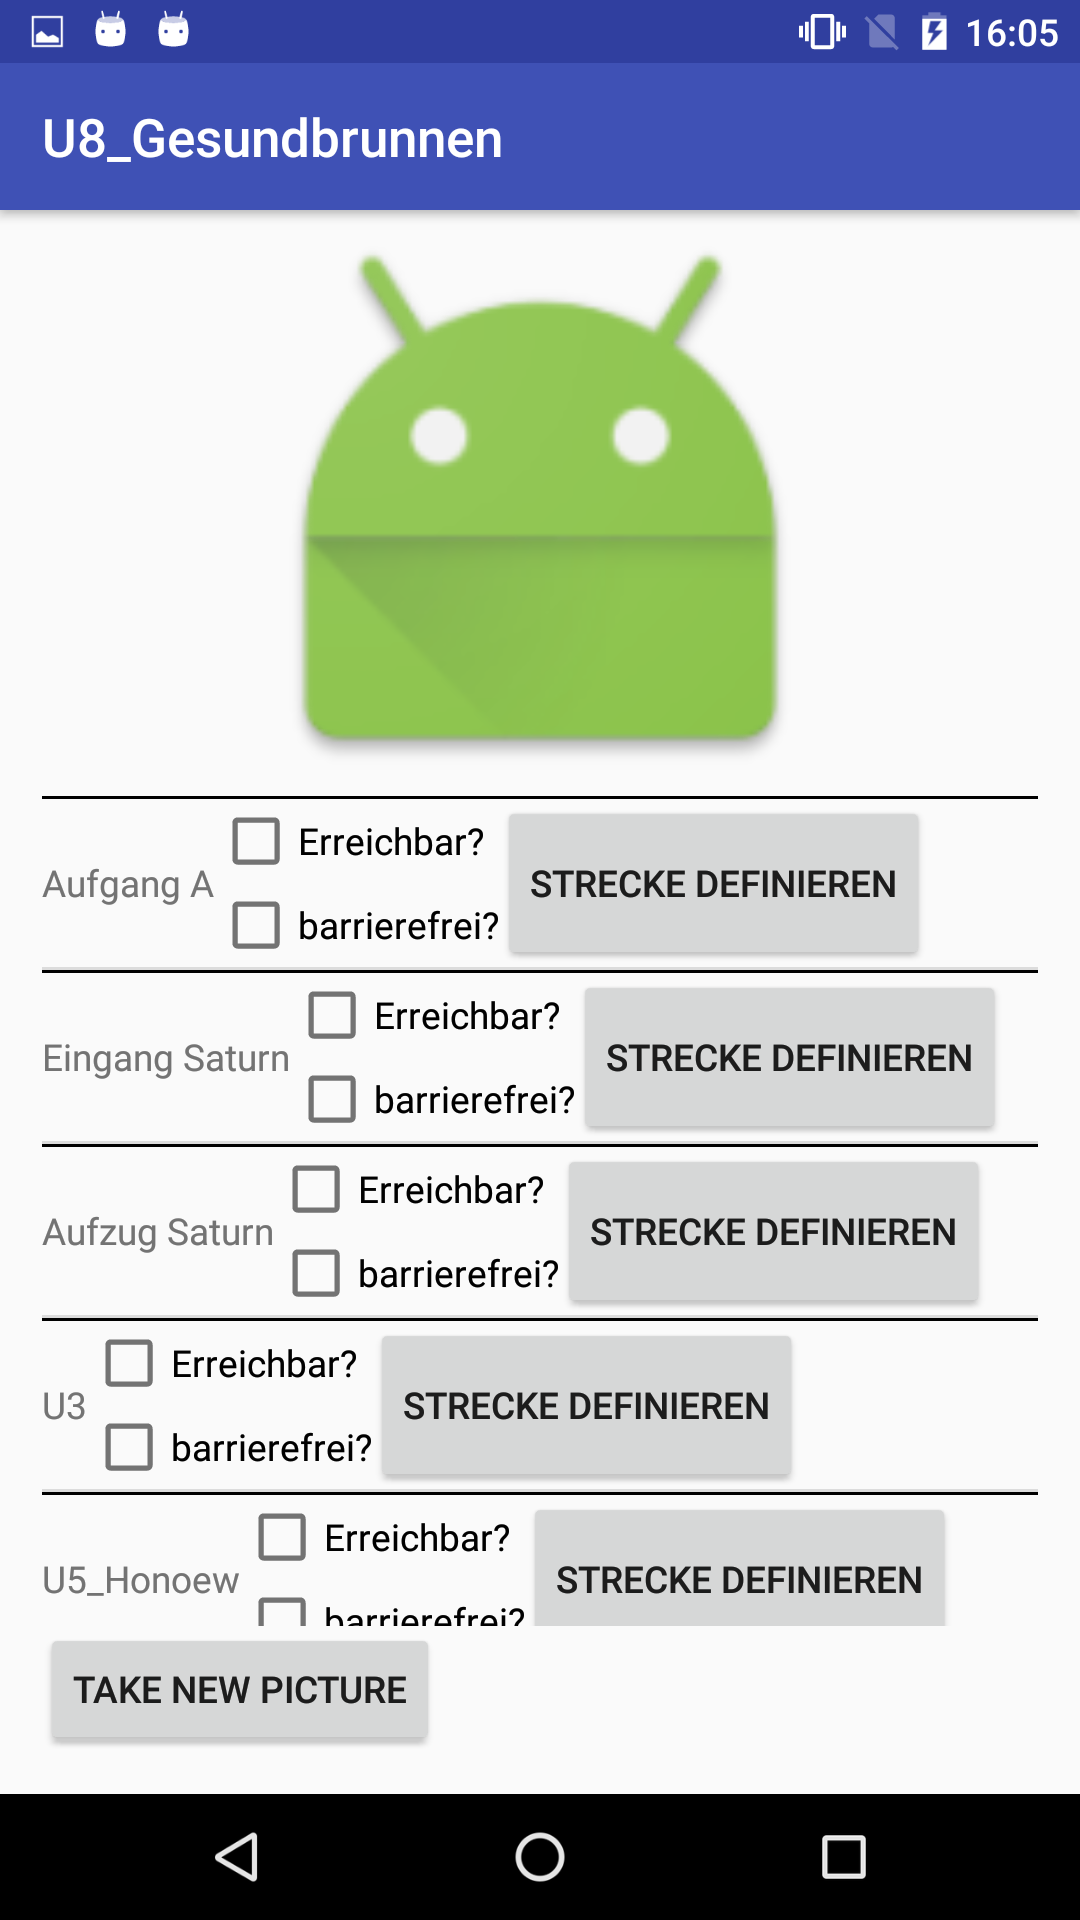
\includegraphics[scale=0.18]{images/poi_gesundbrunnen_details_empty.png}
	\caption{Details von dem POI U5 Gesundbrunnen}
	\label{fig:poi_gesundbrunnen_details_empty}
\end{figure}

Wie es zu sehen ist, hat der POI im Moment noch keine Verbindungen (jede Checkbox "Erreichbar" ist als ungewaehlt markiert).
Da es kein Bild vorhanden ist wird automatisch das Android-Logo angezeigt.

Durch Drucken auf dem "TAKE NEW PICTURE" Knopf kann der Benutzer mit seiner Kamera ein Bild aufnehmen (Bild 5).


\begin{figure}[H]
	\centering
	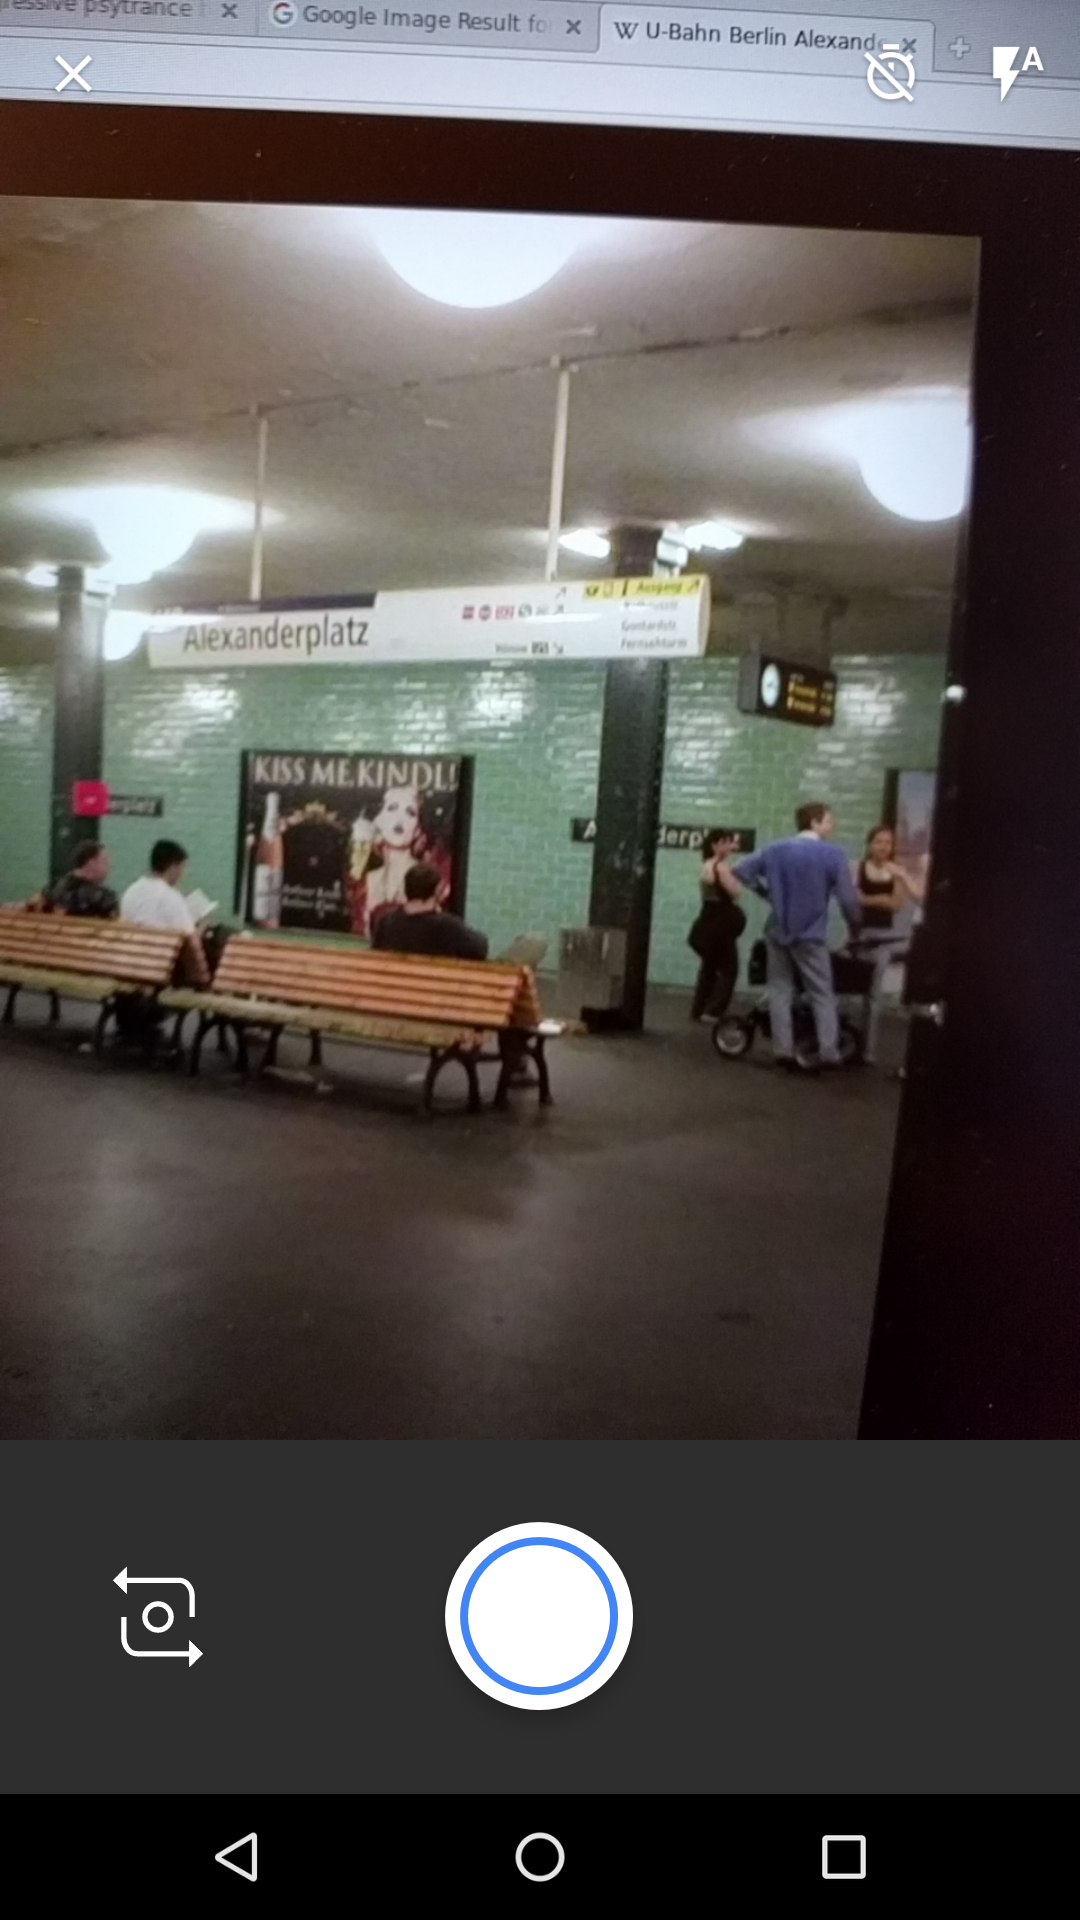
\includegraphics[scale=0.18]{images/poi_gesundbrunnen_take_picture.png}
	\caption{Aufnahme des Bilds fuer den POI U8 Gesundbrunnen}
	\label{fig:poi_gesundbrunnen_take_picture}
\end{figure}

Bei Bestaetigung der Aufnahme wird die vorherige Anzeige mit dem neuen Bild geladen. (Bild 6). Zusaetzlich waehlt der Benutzer in diesem Beispiel den Aufzug neben Saturn als direkte Verbindung.
Die Aenderungen werden auch in den Details des Aufzugs Saturn uebernommen (Bild 7).

\begin{figure}[H]
	\centering
	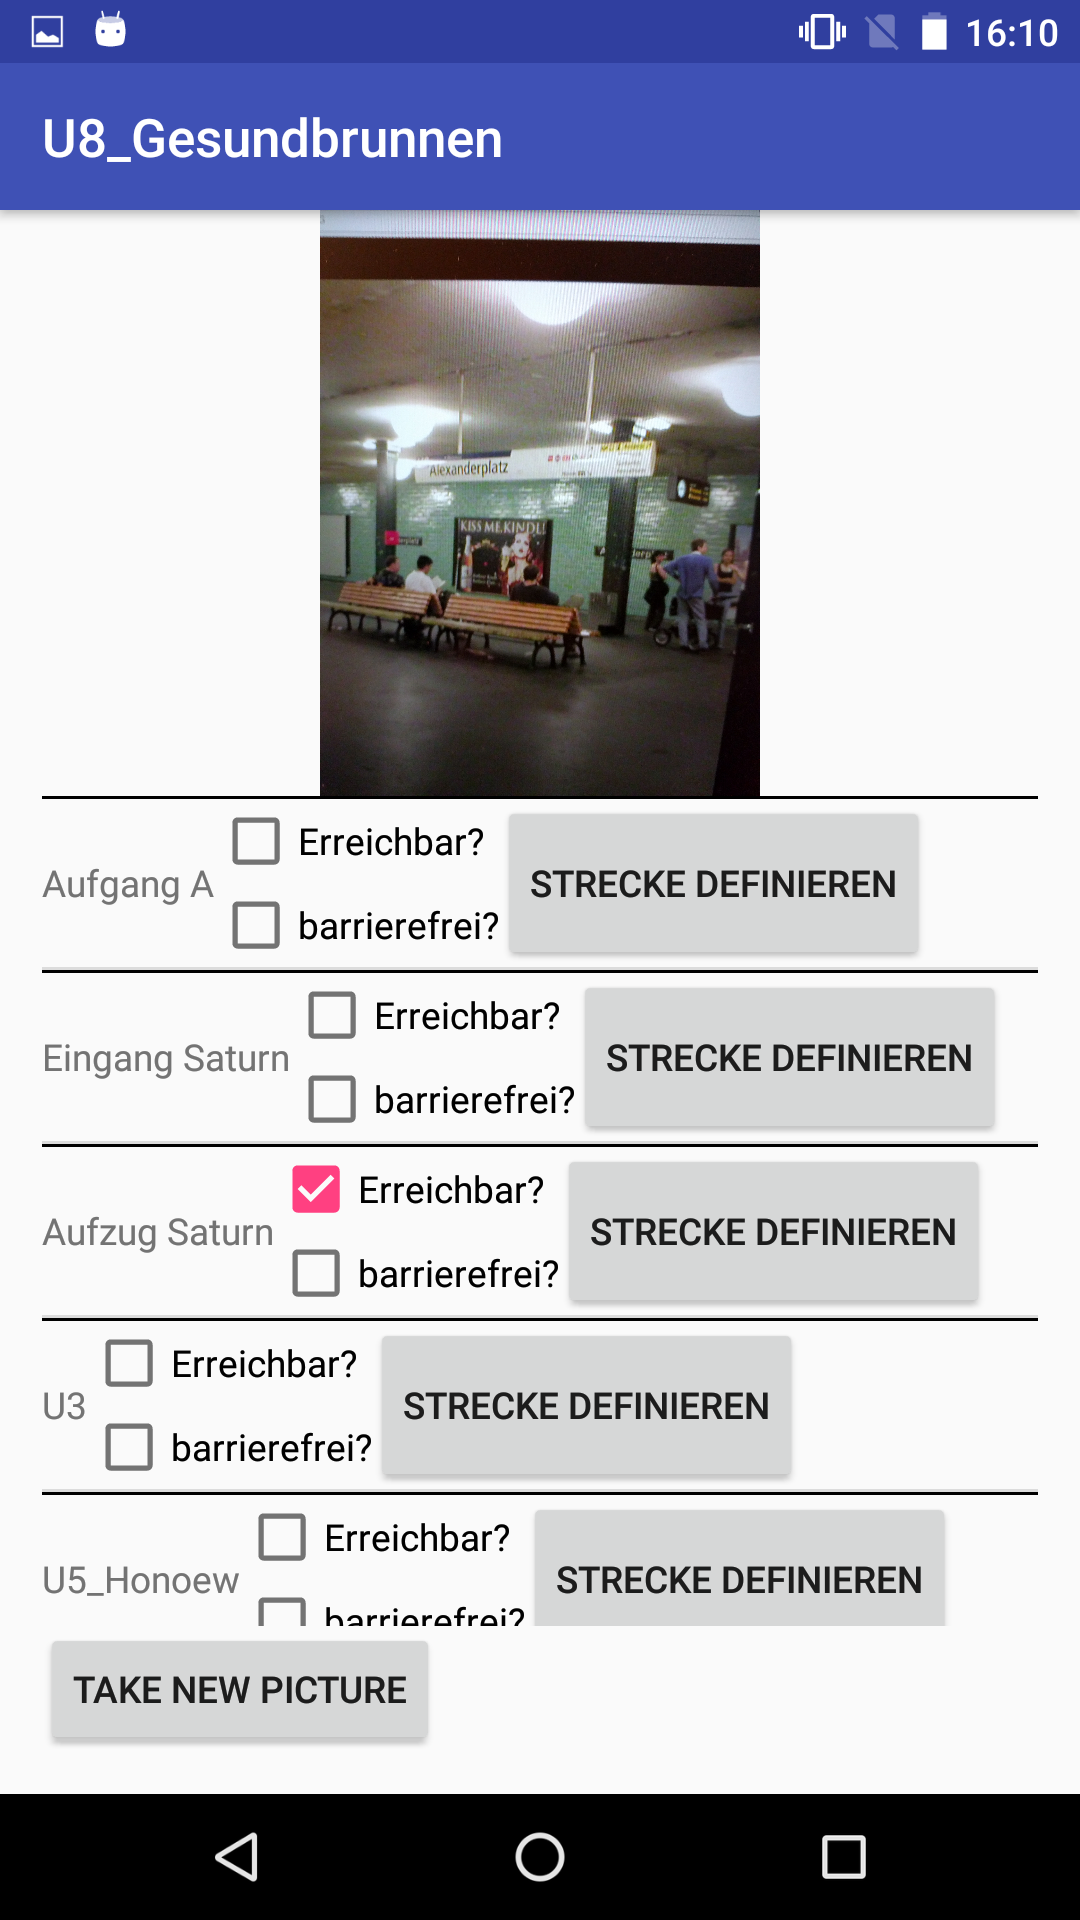
\includegraphics[scale=0.18]{images/poi_gesundbrunnen_picture_taken.png}
	\caption{Details von dem POI U8 Gesundbrunnen mit neuem Bild und gewaehlte direkte Verbindung}
	\label{fig:poi_gesundbrunnen_picture_taken}
\end{figure}


\begin{figure}[H]
	\centering
	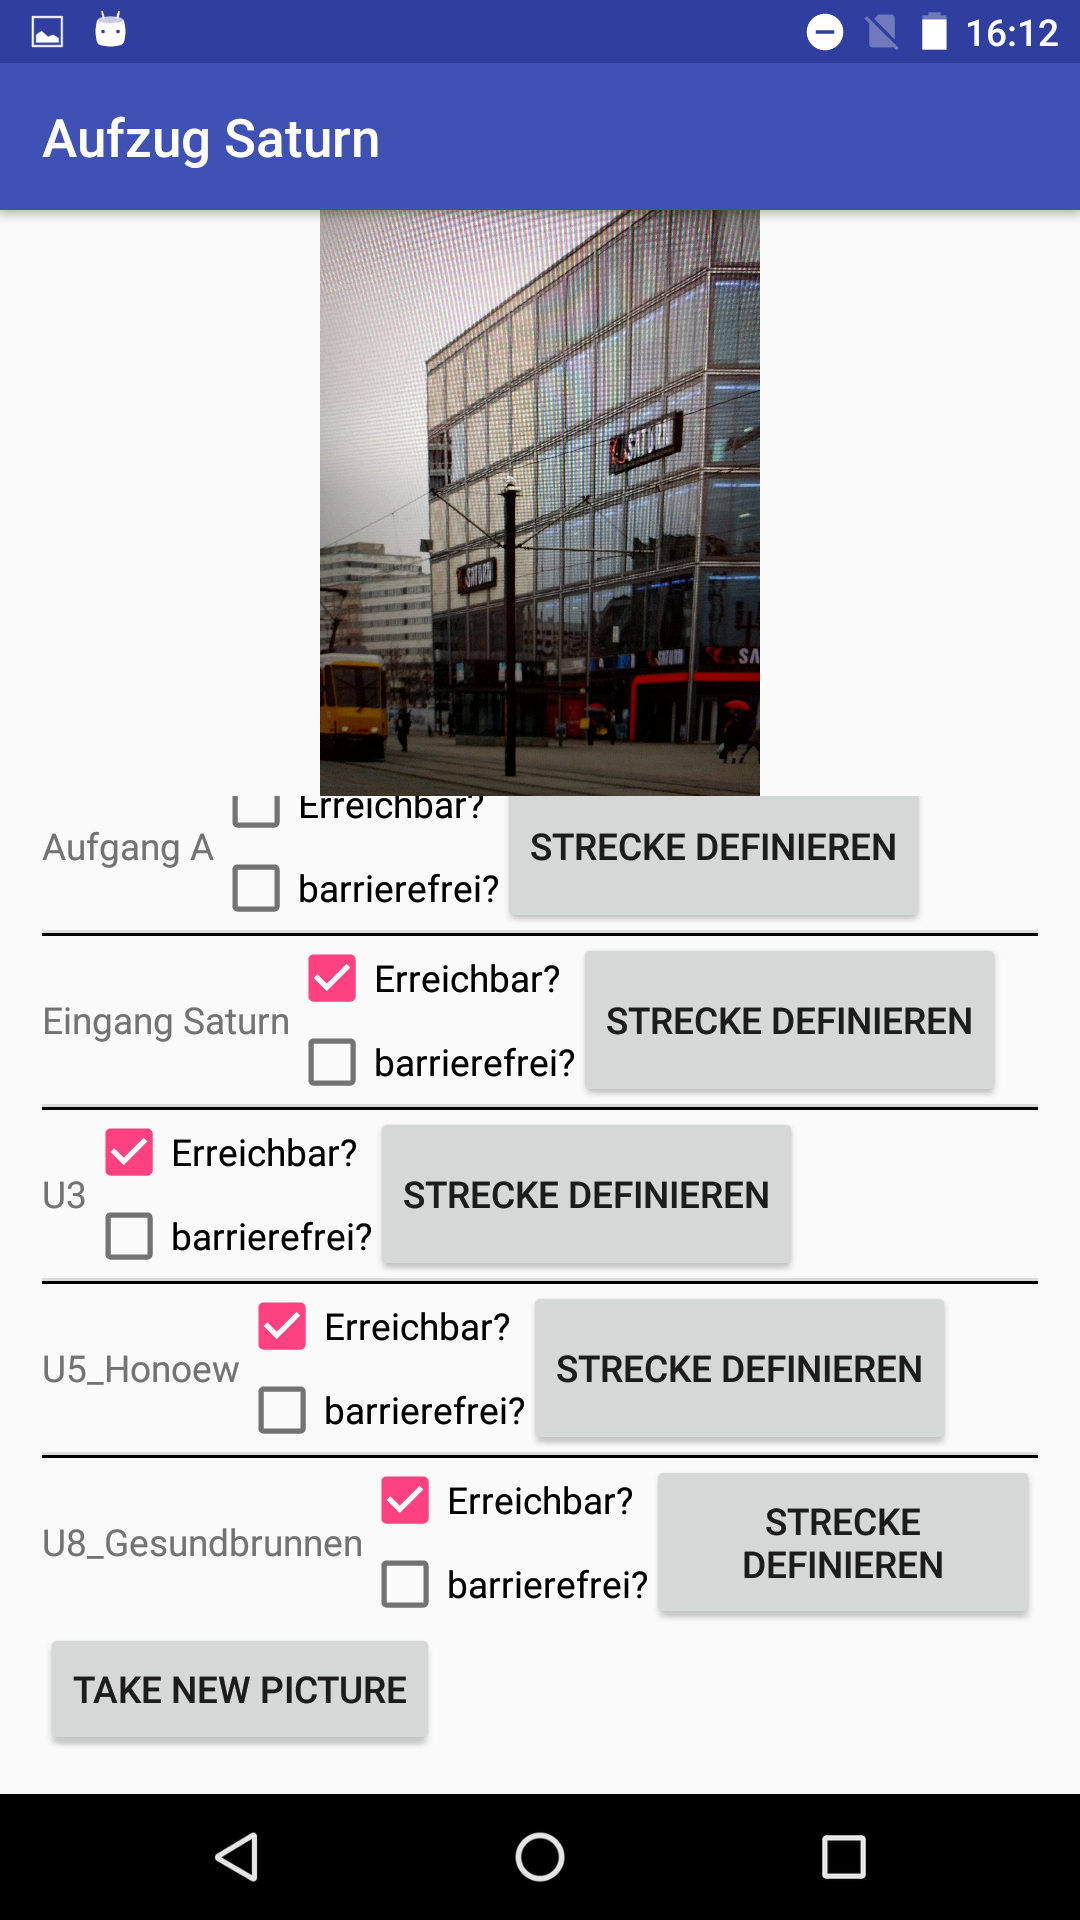
\includegraphics[scale=0.18]{images/poi_aufzug_saturn_details_reflect.png}
	\caption{Details Aufzug Saturn: U8 Gesundbrunnen wird als direkte Verbindung betrachtet}
	\label{fig:poi_aufzug_saturn_details_reflect}
\end{figure}
\subsection*{Kalibrierung der Sensoren, ermitteln der aktuellen Höhe und Distanz}
Es soll Schematisch gezeigt werde wie die Höhe und die ungefähre Distanz ermittelt werden soll.
\begin{figure}[H]
	\centering
	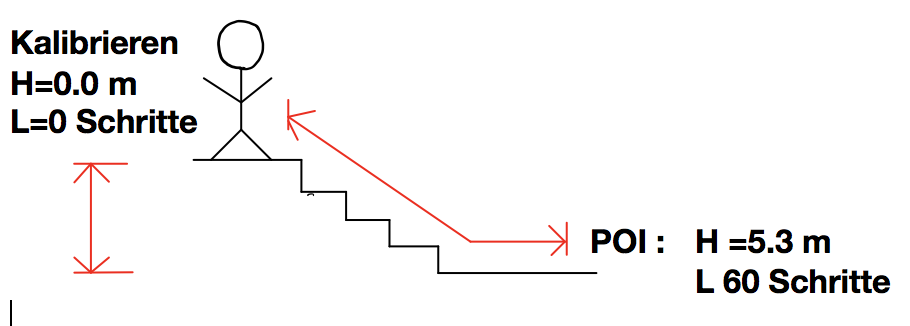
\includegraphics[scale=0.60]{images/skizze-calibration.png}
	\caption{Zeigt wie beim Eingang der U-Bahnstation die Sensoren Kalibriert werden. Von dort an werden die Veränderungen gemessen, stimmen die Sensorwerte mit denen eines POI überein. Kann dies darauf hindeuten das sich der Nutzer dort befindet.}
	\label{fig:skizze-calibration.png}
	
\end{figure}
\begin{figure}[H]
	\centering
	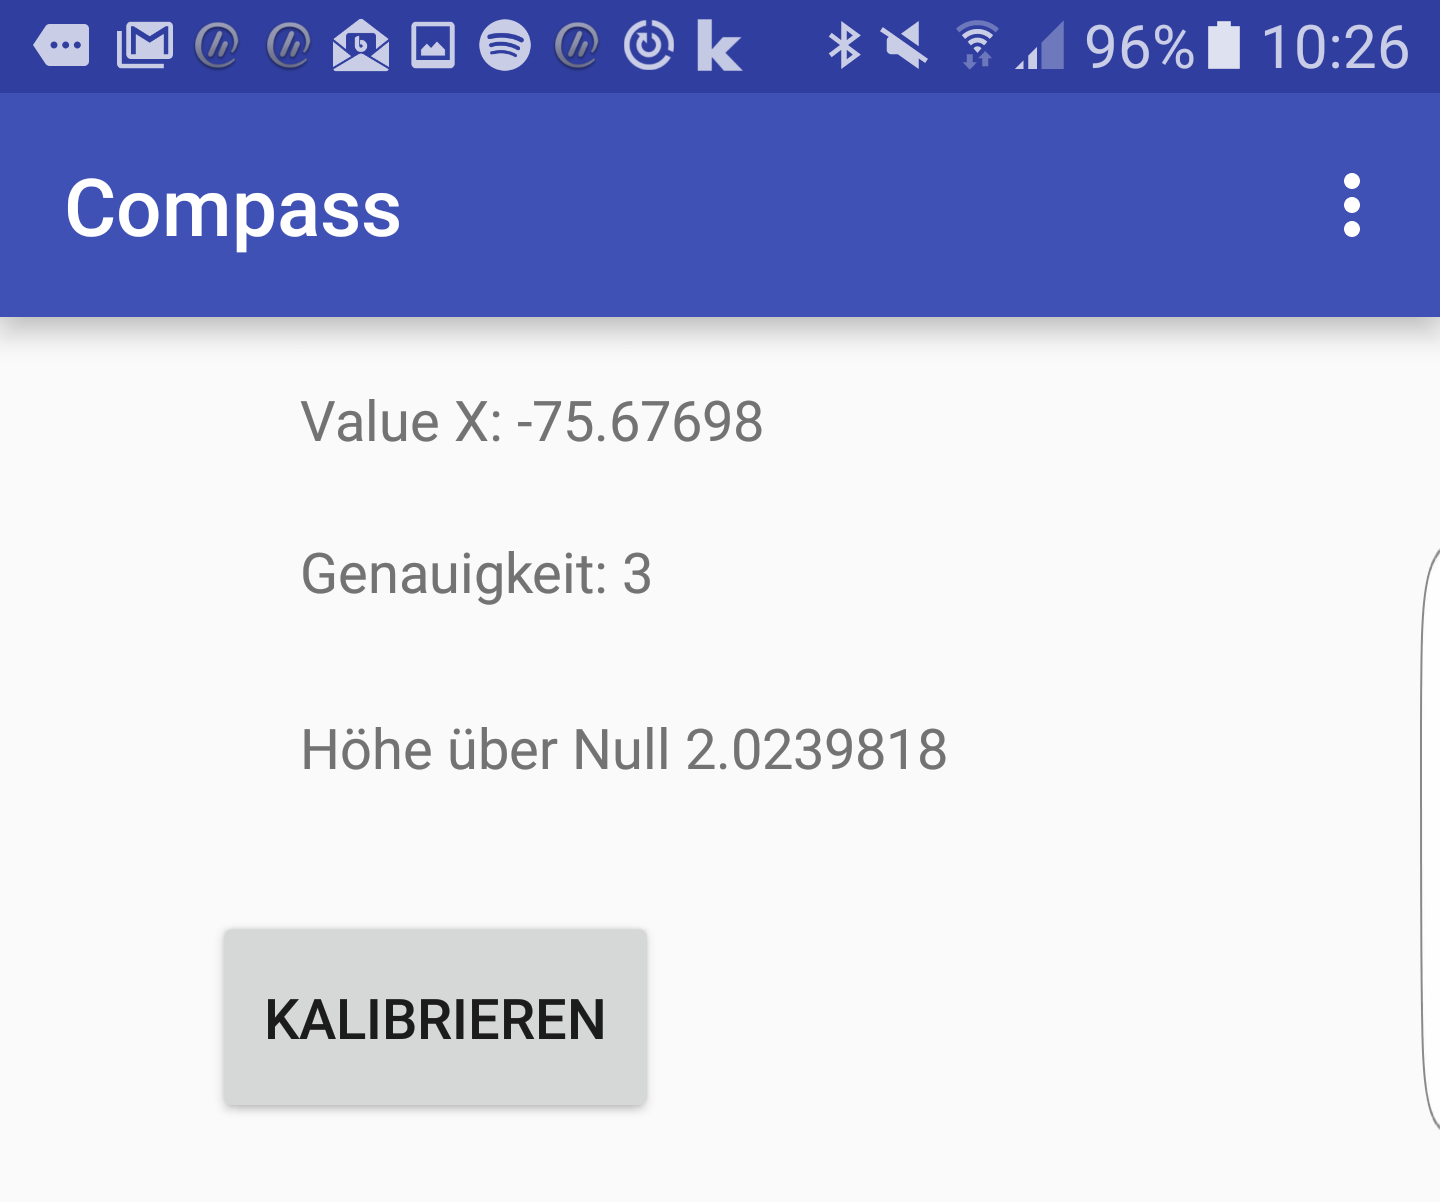
\includegraphics[scale=0.18]{images/app_pic1_calibration.png}
	\caption{Zeigt den  nicht kalibrierten 100 m vor der U-Bahnstation.}
	\label{fig:app_pic1_calibration.png}
\end{figure}
\begin{figure}[H]
	\centering
	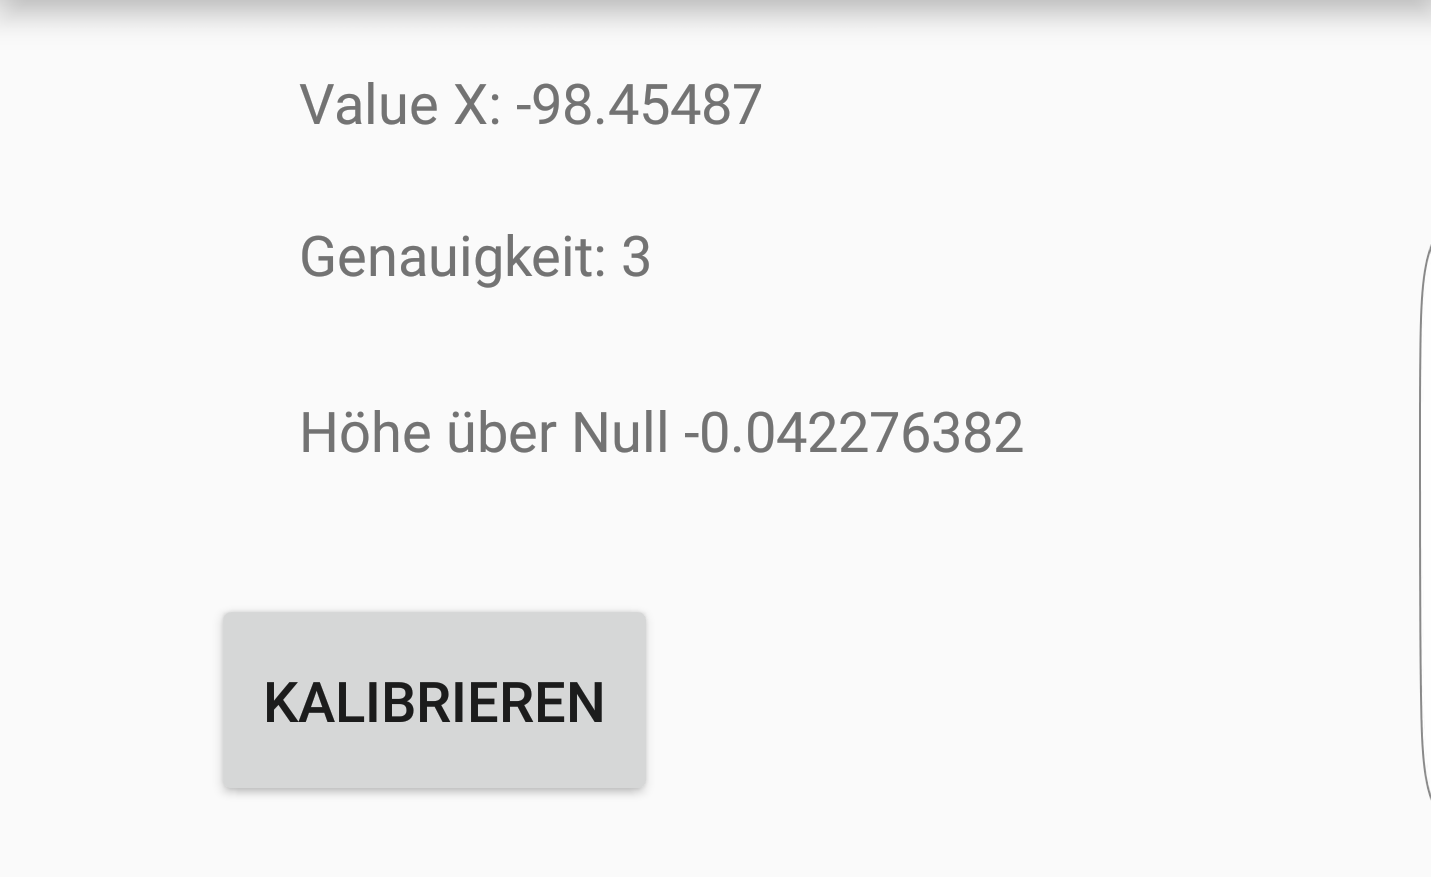
\includegraphics[scale=0.18]{images/app_pic2_calibration.png}
	\caption{Zeigt den kalibrierten Zustand kurz bevor man die U-Bahnstation betritt}
	\label{fig:app_pic2_calibration.png}
\end{figure}



\end{document}
